\section{Introduction}\label{sec:introduction}
%
Robots in today's manufacturing environments typically perform repetitive tasks, and often lack the ability to handle variability and uncertainty. 
Commonly used control algorithms, such as PID regulators and the computed torque method, usually follow predefined trajectories with little adaptive behavior.
Many manufacturing tasks require some degree of adaptability or feedback to the environment, but significant engineering effort and expertise is required to design feedback control algorithms for these industrial robots.
The engineering time for fine tuning such a controller might be similar in cost to the robot hardware itself.
Being able to quickly and easily design feedback controllers for industrial robots would significantly broaden the space of manufacturing tasks that can be automated by robots.

Why is designing a feedback controller for many tasks hard with classical methods? While conventional feedback control methods can solve tasks such as path following efficiently, applications that involve contacts between the robot and its environment are difficult to approach with conventional control methods.
Identifying and characterizing contacts and friction is difficult---even if a physical model provides reasonable contact behavior, identifying the physical parameters of a contact interaction accurately is very hard.
Hence, it is often difficult to achieve adaptable yet robust control behavior, and significant control tuning effort is required as soon as these elements are introduced.
Another drawback of conventional control methods is their lack of behavior generalization.
Thus, all possible system behaviors must be considered a priori at design time.

Reinforcement learning (RL) methods hold the promise of solving these challenges because they allow agents to learn behaviors through interaction with their surrounding environments and ideally generalize to new scenarios that differ from the specifications at the control design stage.
Moreover, RL can handle control problems that are difficult to approach with conventional controllers because the control goal can be specified indirectly as a term in a reward function and not explicitly as the result of a control action.  
All of these aspects are considered enablers for truly autonomous manufacturing systems and important for fully flexible lot-size one manufacturing \citep{lotsizeone}.
However, standard RL methods require the robot learn through interaction, which can be unsafe initially, and collecting the amount of interaction that is needed to learn a complex skill from scratch can be time consuming.

\begin{figure*}[t]
    \vspace{6pt}
    \centering
    \begin{subfigure}[b]{0.45\linewidth}
        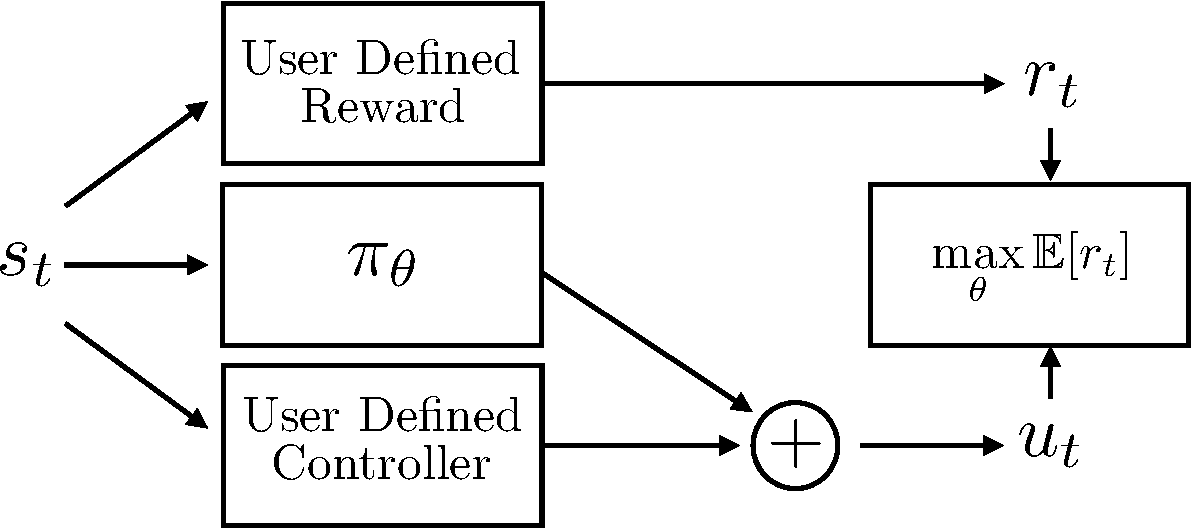
\includegraphics[width=0.9\linewidth]{residualrl/figs/residual_fig1_v4-crop.pdf}
    \end{subfigure}
    \begin{subfigure}[b]{0.54\linewidth}
        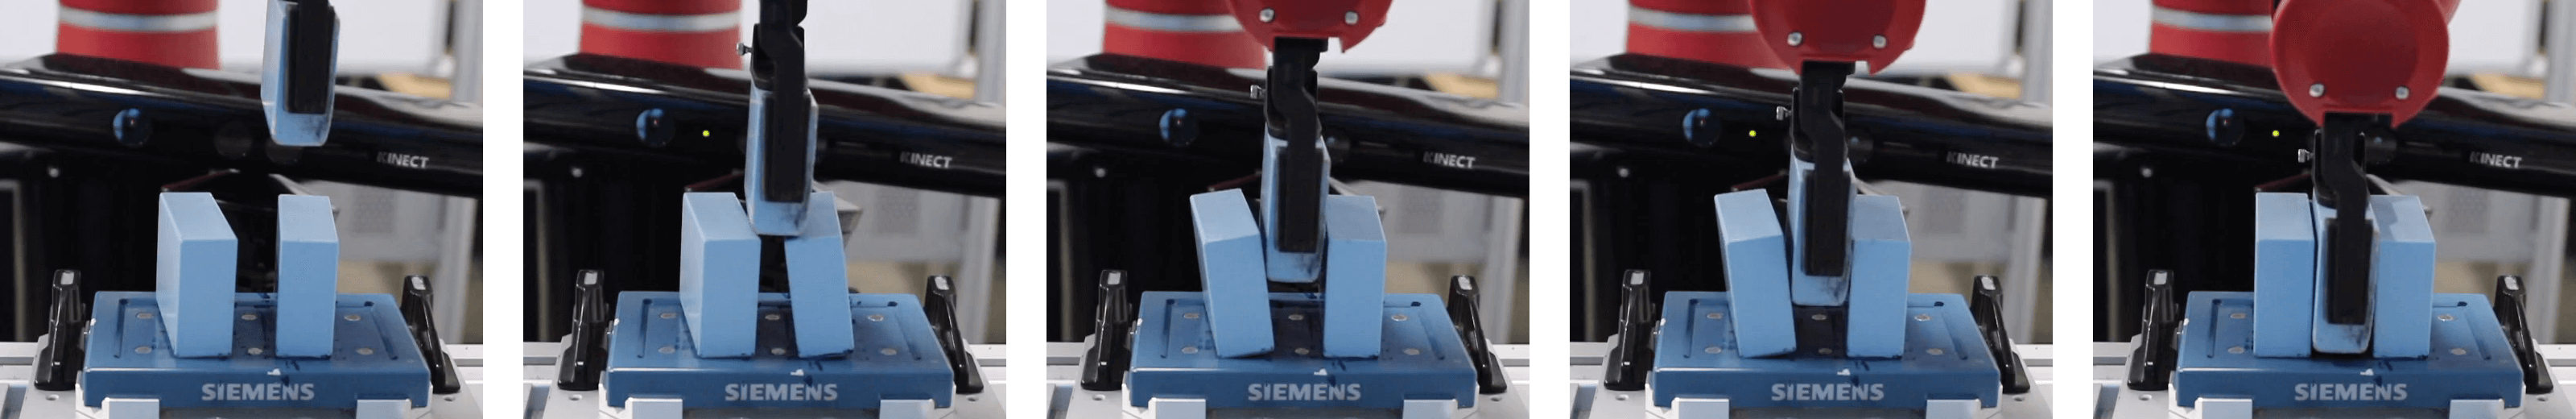
\includegraphics[width=0.99\linewidth]{residualrl/figs/rollout1.png} \\ \\
        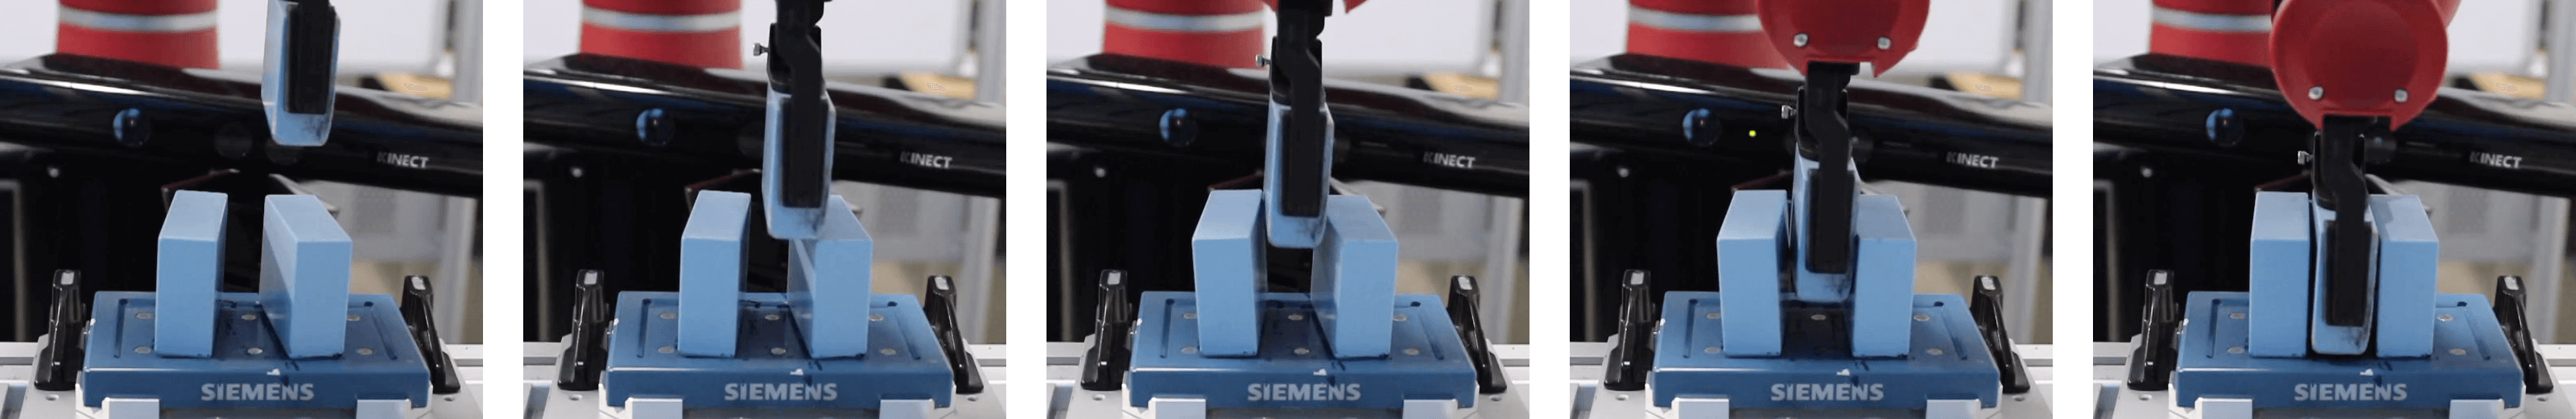
\includegraphics[width=0.99\linewidth]{residualrl/figs/rollout2.png}
    \end{subfigure}
    \caption{We train an agent directly in the real world to solve a model assembly task involving contacts and unstable objects. An outline of our method, which consists of combining hand-engineered controllers with a residual RL controller, is shown on the left. Rollouts of residual RL solving the block insertion task are shown on the right. Residual RL is capable of learning a feedback controller that adapts to variations in the orientations of the standing blocks and successfully completes the task of inserting a block between them. Videos are available at \href{http://residualrl.github.io}{\texttt{residualrl.github.io}}}.
    \label{fig:fig1}
\end{figure*}

In this paper, we study control problems that are difficult to approach with conventional feedback control methods. 
However, the problems possess structure that can be partially handled with conventional feedback control, e.g. with impedance control.
The residual part of the control task, which is the part that must consider contacts and external object dynamics, is solved with RL. The outputs of the conventional controller and RL are superposed to form the commanded control.
The main contribution of this paper is a methodology that combines conventional feedback control with deep RL methods and is illustrated in Fig. \ref{fig:fig1}.
Our main motivation is a control approach that is suitable for real-world control problems in manufacturing, where the exploratory behavior of RL is a safety concern and the data requirements of deep RL can be expensive.
We provide a thorough evaluation of our method on a block assembly task in simulation and on physical hardware. When the initial orientation of the blocks is noisy, our hand-designed controller fails to solve the task, while residual RL successfully learns to perform the task in under 3 hours. This suggests that we could usefully apply our method to practical manufacturing problems.